\begin{figure}[htbp]
	
	\usetikzlibrary{arrows.meta}
	\centering
	\tikzset{
  		point/.style = {% define a style for the function points
    	circle,
    	fill=#1,
    	draw=black,
    	inner sep=2pt,
  	},
  	point/.default = {green!60}
	}

	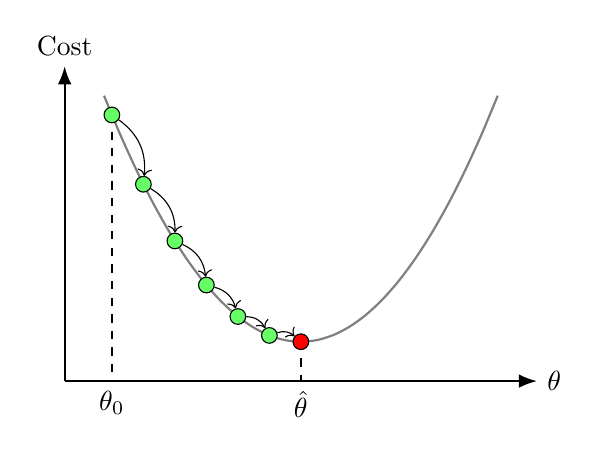
\begin{tikzpicture}[declare function={f(\x)=0.5*\x*\x-3*\x+5;}]
    	\draw[thick,-{LaTeX}](0,0)--(6,0) node[right]{$\theta$};
    	\draw[thick,-{LaTeX}](0,0)--(0,4) node[above]{Cost};
    	\draw[thick, dashed](0.6, {f(0.6)}) -- (0.6,0)
       	   node[below, text width=4em, align=center]{$\theta_0$};
    	\draw[thick, dashed](3, {f(3)}) -- (3,0) node[below]{$\hat\theta$};
    	\draw[domain=0.5:5.5, smooth, thick, gray] plot (\x, f(\x);
    	\foreach \a [count=\c, remember=\c as \C] in {0.6, 1.0, ..., 2.6} {
      	\node[point] (\c) at (\a, {f(\a)}){};
      	\ifnum\c>1 % after the first coordinate draw an arrow
        	 \draw[->, bend left](\C) to (\c);
      	\fi
    	}
    	\node[point=red] (Y) at (3, {f(3)}){}; % add the yellow point
    	\draw[->, bend left](6) to (Y);
 	\end{tikzpicture}
 	\caption{Gradientenverfahren mit zufälligem Startvektor $\theta_0$ und lokalem Minimum $\hat\theta$}
 	\label{fig:gradient_descent}
\end{figure}